\documentclass{article}
\usepackage[utf8]{inputenc} %кодировка
\usepackage[T2A]{fontenc}
\usepackage[english,russian]{babel} %русификатор 
\usepackage{mathtools} %библиотека матеши
\usepackage[left=1cm,right=1cm,top=2cm,bottom=2cm,bindingoffset=0cm]{geometry} %изменение отступов на листе
\usepackage{amsmath}
\usepackage{graphicx} %библиотека для графики и картинок
\graphicspath{}
\DeclareGraphicsExtensions{.pdf,.png,.jpg}
\usepackage{subcaption}
\usepackage{pgfplots}
\usepackage{float}
\usepackage{listings}
\usepackage{hyperref}
\usepackage{physics}

\lstset{
    language=Java,
    frame=single,
    breaklines=true,
    numbers=left, % нумерация строк
    caption={Пример Java кода}, 
    label={lst:java_example}
}

\begin{document}
% НАЧАЛО ТИТУЛЬНОГО ЛИСТА
\begin{center}
    \Large
    Федеральное государственное автономное \\
    образовательное учреждение высшего образования \\ 
    «Научно-образовательная корпорация ИТМО»\\
    \vspace{0.5cm}
    \large
    Факультет программной инженерии и компьютерной техники \\
    Направление подготовки 09.03.04 Программная инженерия \\
    \vspace{1cm}
    \Large
    \textbf{Отчёт по лабораторной работе №4} \\
    По дисциплине «Вычислительная математика» (4 семестр)\\
    \large
    \vspace{8cm}

    \begin{minipage}{.33\textwidth}
    \end{minipage}
    \hfill
    \begin{minipage}{.4\textwidth}
    
        \textbf{Студент}: \vspace{.1cm} \\
        \ Дениченко Александр P3212\\
        \textbf{Практик}:  \\
        \ Наумова Надежда Александровна
    \end{minipage}
    \vfill
Санкт-Петербург\\ 2024 г.
\end{center}
\pagestyle{empty}
% КОНЕЦ ТИТУЛЬНОГО ЛИСТА 
\newpage
\pagestyle{plain}
\section{Цель работы}
Найти функцию, являющуюся наилучшим приближением заданной табличной функции по методу наименьших квадратов.\[\text{Вариант} - 8\]
\section{Вычислительная часть}
1. Сформировать таблицу табулирования заданной функции на указанном интервале (см. табл. 1)\\
2. Построить линейное и квадратичное приближения по 11 точкам заданного интервала;\\
3. Найти среднеквадратические отклонения для каждой аппроксимирующей функции. Ответы дать с тремя знаками после запятой;\\
4. Выбрать наилучшее приближение;\\
5. Построить графики заданной функции, а также полученные линейное и квадратичное приближения;\\
\\
\textbf{Функция по варианту:}
\[y = \frac{3x}{x^4+8},\ x\in [-2,\ 0],\ h=0.2\]
\textbf{График функции:}

\begin{center}
    \begin{figure}[htbp]
        \centering
        \begin{tikzpicture}
        \begin{axis}[
            xlabel={$x$},
            ylabel={$y$},
            xmin=-3, xmax=1,
            ymin=-1, ymax=1,
            grid=both,
            grid style={line width=.1pt, draw=gray!10},
            major grid style={line width=.2pt,draw=gray!50},
            width=16cm,
            height=10cm,
            axis lines=middle,
            enlargelimits={abs=0.5},
            xtick={-3,-2.8,...,1},
            ytick={-1, -0.8, ...,1},
            ticklabel style={font=\footnotesize},
            every axis plot/.append style={line width=1.2pt}
        ]
        
        \addplot[domain=-3:1, samples=100, smooth, blue] {3*x/(x^4+8)};

        \draw[dashed, red, line width=1pt] (axis cs:-2,-1) -- (axis cs:-2,1);
        \draw[dashed, red, line width=1pt] (axis cs:0,-1) -- (axis cs:0,1);

        \end{axis}
        \end{tikzpicture}
        \caption{График функции $y = \frac{3x}{x^4+8}$}
        \label{fig:plot}
        \end{figure}
\end{center}
\textbf{Таблица табулирования функции:}
\begin{center}
    \begin{table}[H]
        \centering
        \begin{tabular}{|c|c|c|c|c|c|c|c|c|c|c|c|}
            \hline
            \( x \) & -2.0 & -1.8 & -1.6 & -1.4 & -1.2 & -1.0 & -0.8 & -0.6 & -0.4 & -0.2 & 0.0 \\
            \hline
            \( y\) & -0.25 & -0.292 & -0.330 & -0.355 & -0.357 & -0.333 & -0.285 & -0.221 & -0.150 & -0.075 & 0.0 \\
            \hline
            \end{tabular}
        \caption{Трассировка}
    \end{table}
\end{center}
\section{Линейная аппроксимация}
Рассмотрим в качестве эмпирической формулы линейную функцию:
\[\phi(a,x,b) = ax + b\]
Сумма квадратов отклонений запишется следующим образом:
\[S = \sum_{i=1}^{n} \varepsilon_i^2 = \sum_{i=1}^{n}(\phi(x_i)-y_i)^2 = \sum_{i=1}^{n}(ax_i^2+b-y_i)^2\ \ ->\ \ min\]
Для нахождения а и b необходимо найти минимум функции S. Необходимое условие существования минимума для функции S:
\begin{equation*}
    \begin{cases}
        \pdv{S}{a} = 0\\
        \pdv{S}{b} = 0
    \end{cases}
    =>
    \begin{cases}
        2\sum_{i=1}^{n}(ax_i+b-y_i)x_i = 0\\
        2\sum_{i=1}^{n}(ax_i+b-y_i) = 0\\
    \end{cases}
    =>
    \begin{cases}
        a\sum_{i=1}^{n}x_i^2+b\sum_{i=1}^{n}x_i = \sum_{i=1}^{n}x_iy_i\\
        a\sum_{i=1}^{n}x_i+bn = \sum_{i=1}^{n}y_i
    \end{cases}
\end{equation*}
Проведём подсчёты:
\[
\sum_{i=1}^{n}x_i = (-2.0) + (-1.8) + (-1.6) + (-1.4) + (-1.2) + (-1.0) + (-0.8) + (-0.6) + (-0.4) + (-0.2) + 0.0 = -11.0
\]
\[
\sum_{i=1}^{n}x_i^2 = (-2.0)^2 + (-1.8)^2 + (-1.6)^2 + (-1.4)^2 + (-1.2)^2 + (-1.0)^2 + (-0.8)^2 + (-0.6)^2 + (-0.4)^2 + (-0.2)^2 + 0.0^2 = 15.4
\]
\[
\sum_{i=1}^{n}y_i = (-0.25) + (-0.292) + (-0.330) + (-0.355) + (-0.357) + (-0.333) + (-0.285) + (-0.221) + (-0.150) + (-0.075) + 0.0 = -2.648
\]
\[
\sum_{i=1}^{n}x_iy_i = (-2.0) \cdot (-0.25) + (-1.8) \cdot (-0.292) + (-1.6) \cdot (-0.330) + (-1.4) \cdot (-0.355) + (-1.2) \cdot (-0.357) + (-1.0) \cdot (-0.333) + (-0.8) \cdot \]
\[\cdot (-0.285) + (-0.6) \cdot (-0.221) + (-0.4) \cdot (-0.150) + (-0.2) \cdot (-0.075) + (0.0) \cdot (0.0) = 3.248
\]
Получим систему:
\begin{equation*}
    \begin{cases}
        15.4a + (-11.0)b = 3.248\\
        -11.0a + 11b = -2.648
    \end{cases}
\end{equation*}
из которой находим:
\[\Delta = 15.4\cdot 11 - 11^2 = 48.4\]
\[\Delta_1 = 3.248\cdot 11 - 11\cdot 2.648 = 6.6\]
\[\Delta_2 = 15.4\cdot (-2.648) - (-11.0)\cdot 3.248 = -5.051\]
Подставим найденные значения:
\[
a = \frac{6.6}{48.4} \approx 0.136; \ \  b = \frac{-5.0512}{48.4}\approx -0.104
\]
Тогда аппроксимирующая функция будет иметь вид:
\[\phi(x) = 0.136x-0.104\]
Дополним таблицу:

\begin{center}
    \begin{table}[H]
        \centering
        \begin{tabular}{|c|c|c|c|c|c|c|c|c|c|c|c|}
            \hline
            \( x \) & -2.0 & -1.8 & -1.6 & -1.4 & -1.2 & -1.0 & -0.8 & -0.6 & -0.4 & -0.2 & 0.0 \\
            \hline
            \( y\) & -0.25 & -0.292 & -0.330 & -0.355 & -0.357 & -0.333 & -0.285 & -0.221 & -0.150 & -0.075 & 0.0 \\
            \hline
            \(\phi(x)\) & -0.377 & -0.350 & -0.323 & -0.295 & -0.268 & -0.241 & -0.214 & -0.186 & -0.159 & -0.132 & -0.105 \\
            \hline
            \(|y-\phi|\)& 0.127& 0.058& 0.007&0.060&0.089&0.092&0.071& 0.035&0.009& 0.057& 0.105\\
            \hline
            \(|y-\phi|^2\)& 0.016& 0.003& 0&0.003&0.007&0.008&0.005&0.001&0& 0.003& 0.011\\
            \hline
        \end{tabular}
        \caption{Линейная аппроксимация}
    \end{table}
\end{center}
Среднеквадратические отклонения по формуле:
\[\delta = \sqrt{\frac{\sum_{i=1}^{n}(\phi(x_i) - y_i)^2}{n}} = 0.0739\]

\section{Квадратичная аппроксимация}

Рассмотрим в качестве эмпирической формулы квадратичную функцию:
\[\phi(x, a_0, a_1, a_2) = a_0 + a_1 x + a_2 x^2\]
Сумма квадратов отклонений записывается следующим образом:
\[S = S(a_0, a_1, a_2) = \sum_{i=1}^{n} (a_0 + a_1 x_i + a_2 x_i^2 - y_i)^2 \rightarrow \min\]
Приравниваем к нулю частные производные \(S\) по неизвестным параметрам, получаем систему линейных уравнений:
\[
\begin{cases}
    \frac{\partial S}{\partial a_0} = 2 \sum (a_2 x_i^2 + a_1 x_i + a_0 - y_i) = 0 \\
    \frac{\partial S}{\partial a_1} = 2 \sum (a_2 x_i^2 + a_1 x_i + a_0 - y_i) x_i = 0 \\
    \frac{\partial S}{\partial a_2} = 2 \sum (a_2 x_i^2 + a_1 x_i + a_0 - y_i) x_i^2 = 0
\end{cases}
\]

\[
\begin{cases}
    a_0 n + a_1 \sum x_i + a_2 \sum x_i^2 = \sum y_i \\
    a_0 \sum x_i + a_1 \sum x_i^2 + a_2 \sum x_i^3 = \sum x_i y_i \\
    a_0 \sum x_i^2 + a_1 \sum x_i^3 + a_2 \sum x_i^4 = \sum x_i^2 y_i
\end{cases}
\]

\[
\sum_{i=1}^{n}x_i = -11.0\ \ 
\sum_{i=1}^{n}x_i^2 = 15.4\ \ 
\sum_{i=1}^{n}y_i = -2.648\ \ 
\sum_{i=1}^{n}x_iy_i = 3.248 \]
\[
\sum_{i=1}^{n}x_i^3 = -24.2\ \ 
\sum_{i=1}^{n}x_i^4 = 40.5328\ \
\sum_{i=1}^{n}x_i^2y_i = -4.62272 \]
Подставим значения:
\[
\begin{cases}
    11\cdot a_0 + (-11.0)\cdot a_1  + 15.4\cdot a_2  = -2.648 \\
    -11.0\cdot a_0 + 15.4\cdot a_1 + (-24.2)\cdot a_2 = 3.248 \\
    15.4\cdot a_0 + (-24.2)\cdot a_1 + 40.5328\cdot a_2 = -4.62272
\end{cases}
\]
Решение системы уравнений:
\[
\begin{cases}
a_0 = 0.02 \\
a_1 = 0.55 \\
a_2 = 0.207
\end{cases}
\]
Получим формулу для квадратичной аппроксимации 
\[\phi(x) = 0.02 + 0.55\cdot x + 0.207\cdot x^2\]

\begin{center}
    \begin{table}[H]
        \centering
        \begin{tabular}{|c|c|c|c|c|c|c|c|c|c|c|c|}
            \hline
            \( x \) & -2.0 & -1.8 & -1.6 & -1.4 & -1.2 & -1.0 & -0.8 & -0.6 & -0.4 & -0.2 & 0.0 \\
            \hline
            \( y\) & -0.25 & -0.292 & -0.330 & -0.355 & -0.357 & -0.333 & -0.285 & -0.221 & -0.150 & -0.075 & 0.0 \\
            \hline
            \(\phi(x)\) &-0.252& -0.299& -0.330& -0.344& -0.341& -0.323& -0.287& -0.235& -0.166& -0.081& 0.02  \\
            \hline
            \(|y-\phi|\)&0.002& 0.007& 0& 0.01072& 0.015& 0.01& 0.002& 0.014& 0.016& 0.006& 0.02 \\
            \hline
            \(|y-\phi|^2\cdot 10^{-4}\)&0.04&5&0.006&1.14&2.27&1&0.063&2.09&2.84&0.451&4\\
            \hline
        \end{tabular}
        \caption{Квадратичная аппроксимация}
    \end{table}
\end{center}
Среднеквадратические отклонения по формуле:
\[\delta = \sqrt{\frac{\sum_{i=1}^{n}(\phi(x_i) - y_i)^2}{n}} = 0.011\]
\section{Построения результатов}
Исходная:
\[y = \frac{3x}{x^4+8}\]
Линейная:
\[\zeta(x) = 0.136x-0.104\]
Квадратичная:
\[\aleph(x) = 0.02 + 0.55\cdot x + 0.207\cdot x^2\]



\begin{center}
    \begin{figure}[htbp]
        \centering
        \begin{tikzpicture}
        \begin{axis}[
            xlabel={$x$},
            ylabel={$y$},
            xmin=-3, xmax=1,
            ymin=-1, ymax=1,
            grid=both,
            grid style={line width=.1pt, draw=gray!10},
            major grid style={line width=.2pt,draw=gray!50},
            width=16cm,
            height=10cm,
            axis lines=middle,
            enlargelimits={abs=0.5},
            xtick={-3,-2.8,...,1},
            ytick={-1, -0.8, ...,1},
            ticklabel style={font=\footnotesize},
            every axis plot/.append style={line width=1.2pt}
        ]
        
        
        % Линейная функция
        \addplot[domain=-3:1, samples=100, smooth, blue] {0.136*x-0.104};
        \addlegendentry{$\zeta=0.136x-0.104$}

        % Квадратичная функция
        \addplot[domain=-3:1, samples=100, smooth, pink] {0.02 + 0.55*x + 0.207*x^2};
        \addlegendentry{$\aleph=0.02 + 0.55x + 0.207x^2$}

        % Рациональная функция
        \addplot[domain=-3:1, samples=100, smooth, green] {3*x/(x^4+8)};
        \addlegendentry{$y=\frac{3x}{x^4+8}$}

        \draw[dashed, red, line width=1pt] (axis cs:-2,-1) -- (axis cs:-2,1);
        \draw[dashed, red, line width=1pt] (axis cs:0,-1) -- (axis cs:0,1);

        \end{axis}
        \end{tikzpicture}
        \caption{Графики для сравнения}
        \label{fig:plot}
        \end{figure}
\end{center}
Самое хорошее приближении получилось квадратичное, оно наиболее чётко совпадает с графиком исходной функции в системе декартовых координат.







\section{Машинная реализация}

\begin{lstlisting}[language=Java, caption={Первый узел валидации}]
private CalculateError isValidInterval(RequestFuncUser requestFuncUser) {
    
\end{lstlisting}


 
\section{Пример работы программы}


\section{GitHub}
Ссылка на мой репозиторий на GitHub: \url{https://github.com/Alex-de-bug/cm_math/tree/main/lab3}.

\section{Вывод}
При работе были изучены несколько численных методов вычисления интегралов, написаны несколько алгоритмов для реализации. Подсчёт руками помог усвоить все тонкости работы численных методов. Придумана обработка точек разрыва в том числе неустранимых 2го рода.
\end{document}
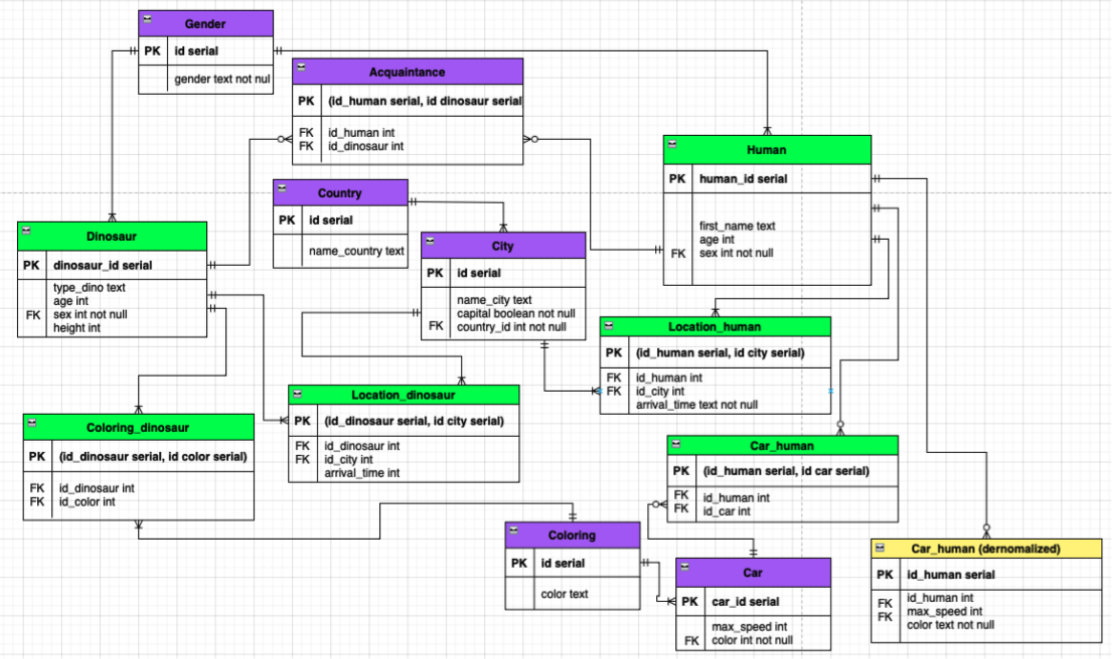
\includegraphics[width=.9\textwidth]{123}